
\subsection{Box-in-box AMR}
\label{sec:box_in_box_amr}
\CarpetX\space supports fixed mesh refinement via the so called box-in-box paradigm. This capability is provided by the \texttt{BoxInBox} thorn. Using it is very simple and similar to \texttt{Carpet}'s \texttt{CarpetRegrid2} usage.

\begin{table}[ht]
  \resizebox{\columnwidth}{!}{%
    \begin{tabular}{ccccc}
    Name                    & Type                      & Possible Values                                                   & Default Value                   & Description                               \\\hline\hline
    \texttt{shape\_n}       & String                    & \texttt{"sphere"} or \texttt{"cube"}                              & \texttt{"sphere"}               & Shape of refined region                   \\
    \texttt{active\_n}      & Boolean                   & \texttt{"yes"} or \texttt{"no"}                                   &  \texttt{"yes"}                 & Is this box active?                       \\
    \texttt{num\_levels\_n} & Single integer             & $[1,30]$                                                          & $1$                             & Number of refinement levels for this box  \\
    \texttt{position\_x\_n} & Single real number        & Any real                                                          & $0.0$                           & x-position of this box                    \\
    \texttt{position\_y\_n} & Single real number        & Any real                                                          & $0.0$                           & y-position of this box                    \\
    \texttt{position\_z\_n} & Single real number        & Any real                                                          & $0.0$                           & z-position of this box                    \\
    \texttt{radius\_n}      & 30 element array of reals & $-1.0$ or positive real                                           & $-1.0$ (radius ignored)         & Radius of refined region for this level   \\
    \texttt{radius\_x\_n}   & 30 element array of reals & $-1.0$ or positive real                                           & $-1.0$ (radius ignored)         & x-radius of refined region for this level \\
    \texttt{radius\_y\_n}   & 30 element array of reals & $-1.0$ or positive real                                           & $-1.0$ (radius ignored)         & y-radius of refined region for this level \\
    \texttt{radius\_z\_n}   & 30 element array of reals & $-1.0$ or positive real                                           & $-1.0$ (radius ignored)         & z-radius of refined region for this level \\\hline\hline
  \end{tabular}%
  }
  \caption{Configuration parameters for a single (1 out of 3) box that can be defined in parameter files using the \texttt{BoxInBox} thorn.}
  \label{tab:box_config}
\end{table}

All configuration of boxes and levels are performed within configuration files. \texttt{BoxInBox} supports adding 3 ``boxes'' or ``centers''. Each box can be configured as summarized in Tab.~\ref{tab:box_config}. The \texttt{n} suffix should be replaced by \texttt{1}, \texttt{2} or \texttt{3} for configuring the corresponding boxes. Each box can be shaped differently as either Cartesian-like cubes or spheres and support configuring up to 30 levels. Level's positions and radii can be set independently for each dimension. Note that for each box the \texttt{active}, \texttt{num\_levels} and \texttt{position\_(xyz)} field are stored as grid scalars. Each of the 30 refinement level radii and \texttt{x, y, z} individual radii for each box are also stored as grid arrays. This allows these parameters to be changed during a simulation run, allowing for moving boxes. This is useful, for example, when implementing a puncture tracker. 

These configurations are subjected to (and restricted by) two additional \CarpetX\space configurations, namely \texttt{CarpetX::regrid\_every}, which controls how many iterations should pass before checking if the box grid variables have changed and \texttt{CarpetX::max\_num\_levels} which controls the maximum number of allowed refinement levels.

As an example, we present a configuration file excerpt for creating two refinement boxes with the \texttt{BoxInBox} thorn

\begin{lstlisting}[language=bash]
  BoxInBox::num_regions = 2

  BoxInBox::num_levels_1 = 2
  BoxInBox::position_x_1 = -0.5
  BoxInBox::radius_x_1[1] = 0.25
  BoxInBox::radius_y_1[1] = 0.25
  BoxInBox::radius_z_1[1] = 0.25

  BoxInBox::num_levels_2 = 2
  BoxInBox::position_x_2 = +0.5
  BoxInBox::radius_x_2[1] = 0.25
  BoxInBox::radius_y_2[1] = 0.25
  BoxInBox::radius_z_2[1] = 0.25
\end{lstlisting}

Let us now suppose that one wishes to make the boxes set up in the above parameter file to move in a circle around the origin. This is not very useful in practice, but it illustrates important concepts that can be later applied to more complex tools, such as puncture trackers. The \texttt{MovingBoxToy} thorn bundled in \CarpetX\space provides an example of how to achieve this. We shall now examine this implementation closely. Let us start by the examining the thorn's \texttt{interface.ccl} file:
%
\begin{lstlisting}[language=bash]
  # Interface definition for thorn MovingBoxToy

  IMPLEMENTS: MovingBoxToy

  INHERITS: BoxInBox
\end{lstlisting}

The \texttt{INHERITS} statement in line 5 states that this thorn will write to grid functions provided in \texttt{BoxInBox} which control the refinement boxes parameters. Next, in the thorn's \texttt{param.ccl} file we have
%
\begin{lstlisting}
  # Parameter definitions for thorn MovingBoxToy

  shares: BoxInBox
  USES CCTK_REAL position_x_1
  USES CCTK_REAL position_x_2
\end{lstlisting}

Lines 3-5 declare that \texttt{MovingBoxToy} uses parameters \texttt{position\_x\_1} and \texttt{position\_x\_2} from \texttt{BoxInBox}. These declarations are required in order to access the initial positions of the boxes. Note that similar statements would be used if other parameters from \texttt{BoxInBox} were required.

Finally, in the \texttt{schedule.ccl} file we schedule the routine that will actually update the box positions, called \texttt{MovingBoxToy\_MoveBoxes}:
%
\begin{lstlisting}
  # Schedule definitions for thorn MovingBoxToy

  SCHEDULE MovingBoxToy_MoveBoxes AT postinitial BEFORE EstimateError
  {
    LANG: C
    READS: BoxInBox::positions
    WRITES: BoxInBox::positions
  } "Update box positions"

  SCHEDULE MovingBoxToy_MoveBoxes AT poststep BEFORE EstimateError
  {
    LANG: C
    READS: BoxInBox::positions
    WRITES: BoxInBox::positions
  } "Update box positions"
\end{lstlisting}

Note that the routine is scheduled with \texttt{AT poststep BEFORE EstimateError}. This is important, since it is in the \texttt{EstimateError} bin that \CarpetX's AMR error grid function (see Sec.~\ref{sec:advanced_amr}) will be updated thus any changes to box data should be scheduled before that.

Finally, the \texttt{C++} routine \texttt{MovingBoxToy\_MoveBoxes} that will actually update the boxes positions reads
%
\begin{lstlisting}
  extern "C" void MovingBoxToy_MoveBoxes(CCTK_ARGUMENTS) {
    DECLARE_CCTK_ARGUMENTSX_MovingBoxToy_MoveBoxes;
    DECLARE_CCTK_PARAMETERS;

    using std::cos;

    const CCTK_REAL omega{M_PI/4};

    // Initial positions of box 1
    const auto x0_1{position_x_1};

    // Initial positions of box 2
    const auto x0_2{position_x_2};

    // Trajectory of box 1
    position_x[0] = x0_1 * cos(omega * cctk_time);
    position_y[0] = x0_1 * sin(omega * cctk_time);

    // Trajectory of box 2
    position_x[1] = x0_2 * cos(omega * cctk_time);
    position_y[1] = x0_2 * sin(omega * cctk_time);
  }
\end{lstlisting}

In lines 10 and 13, we read \texttt{BoxInBox} parameters for the initial positions of the boxes. In line 16-21 those positions are updated in a way that the boxes centers describe a circle around the origin. At each time, the boxes move $\pi/4$ radians around the origin in a counterclockwise fashion. Figure~\ref{fig:boxes_circle} shows 6 still frames of the boxes motions around the origin. All panels are $z=0$ slices of the grid hierarchy and time and iteration values are provided for each panel. These plots were produced with the \texttt{VisIt} visualization software with \CarpetX\space producing \texttt{silo} data files as output (see Sec.~\ref{sec:data} for more details on how to visualize and post-process \CarpetX\space data). The data can be reproduced by running the \texttt{circle.par} parameter file, provided in the \texttt{par} folder of the \texttt{MovingBoxToy} thorn. An animated version of Fig.~\ref{fig:boxes_circle} can be found in the \texttt{doc} folder of the \CarpetX\space thorn under the name {animated\_boxes.gif}.

\begin{figure*}[ht]
  \begin{center}
      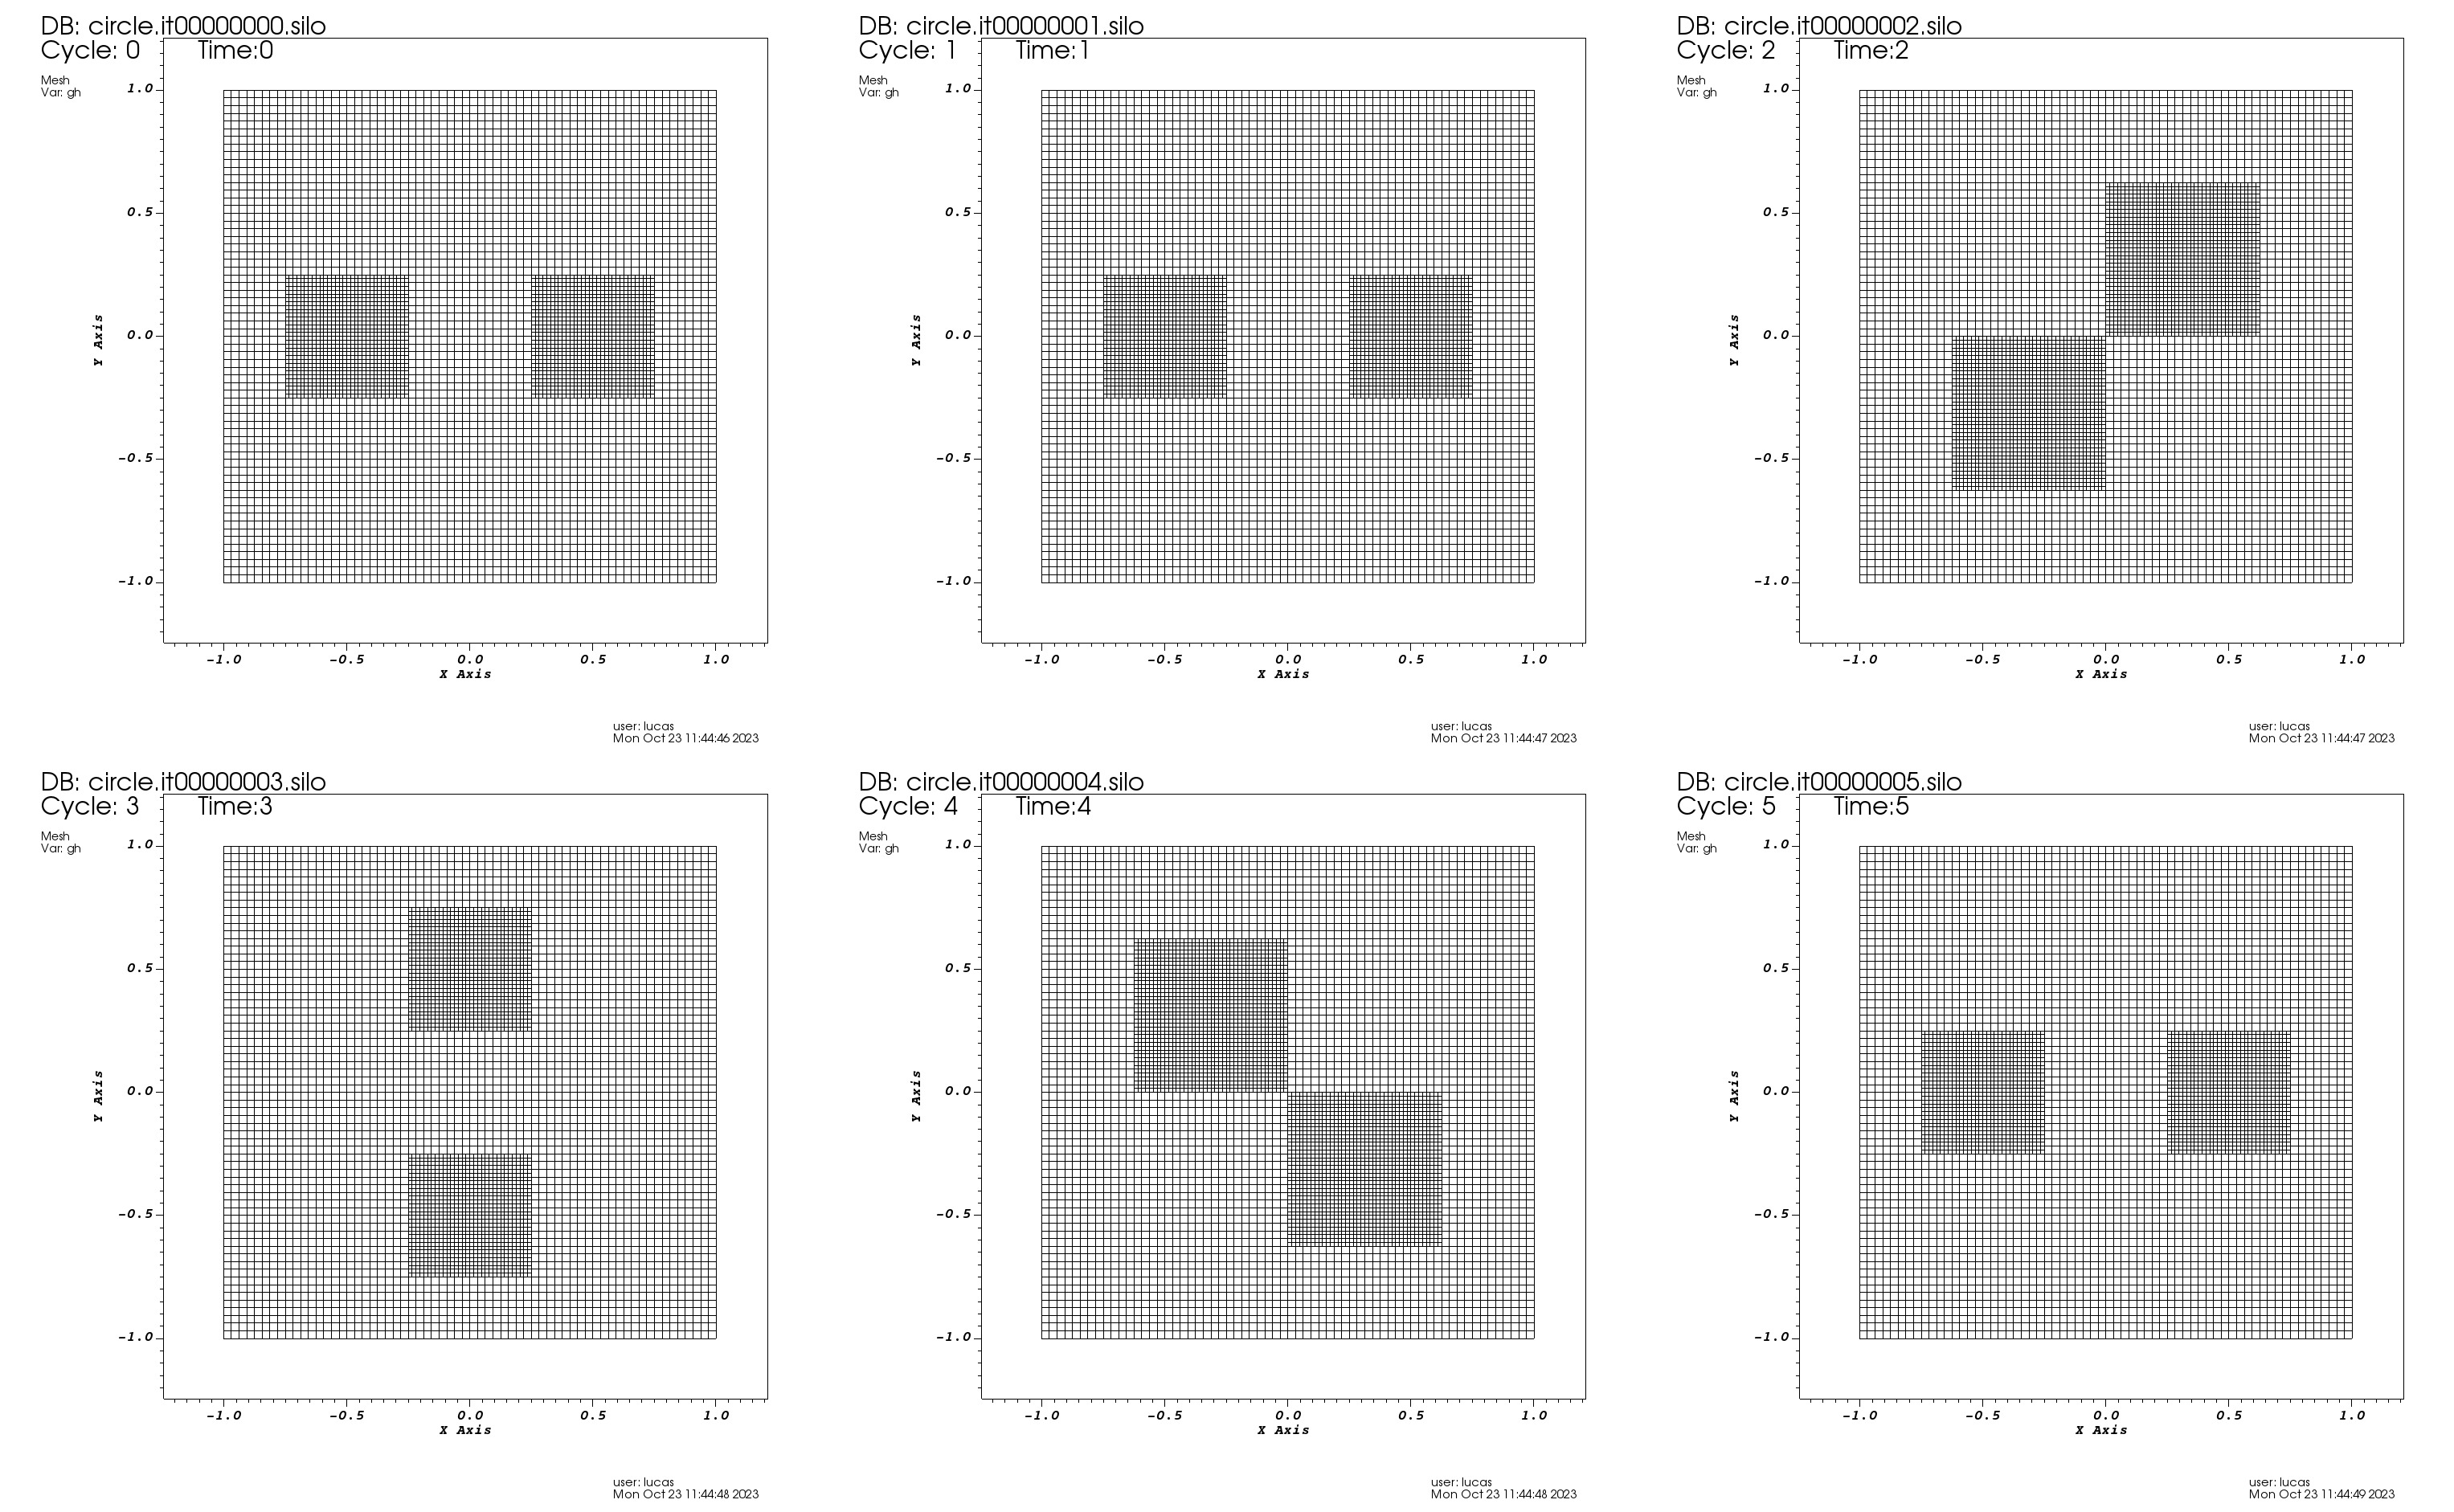
\includegraphics[width=\linewidth]{boxes_frames.png}
  \end{center}
  \caption{AMR boxes moving around a circle, as implemented in the \texttt{MovingBoxToy} thorn.}
  \label{fig:boxes_circle}
\end{figure*}

\subsection{Advanced AMR}
\label{sec:advanced_amr}

\CarpetX\space supports non-fixed (adaptive) mesh refinement. For cell level control of AMR, \CarpetX\space provides user with a cell centered and non-checkpointed grid function called \texttt{regrid\_error}. Users are responsible for filling this grid function with real value however they see fit. Once it is filled, the configuration parameter \texttt{CarpetX::regrid\_error\_threshold} controls regridding: If the values stored in \texttt{regrid\_error} are larger than what is set in \texttt{regrid\_error\_threshold}, the region gets refined. Additionally, the configuration parameter \texttt{CarpetX::regrid\_every} controls how many iterations should pass before checking if the error threshold has been exceeded. The parameter \texttt{CarpetX::max\_num\_levels} controls the maximum number of allowed refinement levels.

Note that \CarpetX\space \textbf{does not} provide a ``standardized'' regrid error routine. This is because refinement criteria are highly specific to the problem being solved via AMR, and thus there is no one size fits all error criteria. This might seem inconvenient, but ultimately it allows for users to have higher degrees of customization in their AMR codes. For demonstration purposes, we shall now provide a routine that estimates the regrinding error as \todo{what? Provide a good starter example}. This implementation could be used as a starting point for codes that wish to use different error criteria in their AMR grids.

\begin{lstlisting}
  extern "C" void EstimateError(CCTK_ARGUMENTS) {
  DECLARE_CCTK_ARGUMENTSX_EstimateError;
  DECLARE_CCTK_PARAMETERS;

  // The template indices indicate this a loop over cell centers
  // Remember that regrid_error is a cell centered grid function
  grid.loop_int_device<1, 1, 1>(
      grid.nghostzones,
      [=] (const Loop::PointDesc &p) {
        // TODO: Give a simple example
        regrid_error(p.I) = 0.0;
      });
}
\end{lstlisting}

Once defined, \texttt{EstimateError} should be scheduled in both the \texttt{postinitial} and \texttt{poststep} bins. The \texttt{poststep} bin gets called right after a new state vector has been calculated, and is thus the proper place to analyze it. The \texttt{postinitial} scheduling is also necessary for computing the initial refinement after initial conditions have been set up. A thorn making use of the \texttt{regrid\_error} AMR mechanism should then add the following to its \texttt{schedule.ccl} file:

\begin{lstlisting}[language=bash]
  SCHEDULE EstimateError AT postinitial
  {
    LANG: C
    READS: state(everywhere)
    WRITES: CarpetX::regrid_error(interior)
  } "Estimate error for regridding"
  
  SCHEDULE EstimateError AT poststep
  {
    LANG: C
    READS: state(everywhere)
    WRITES: CarpetX::regrid_error(interior)
  } "Estimate error for regridding"
\end{lstlisting}
